\chapter{ロバスト最適化}
\label{chap::robust}

\hspace{1zw}本章では,外気温の予報と実際の差異に対処するためのロバスト最適化の試みについて述べる.

\section{概要}
最適化システムの構成を\figref{fig::robust_system}に示す.前章のシステムと同様に,評価部では,EnergyPlusシミュレーションを用いる.前章のシステムとの違いは,目的関数である.外気温予報に誤差がない場合の室内快適性に関する第1目的関数$f_1$, エネルギー消費量に関する第2目的関数$f_2$に加え,外気温予報に誤差がある場合の快適性の変動幅に関する第3目的関数$f_3$とエネルギー消費量の変動幅に関する第4目的関数$f_4$を考慮する.これら4つの目的関数を最適化することによって,外気温予報の誤差にロバストな空調設定スケジュールを得る.

\begin{figure*}[t]
    \begin{center}
        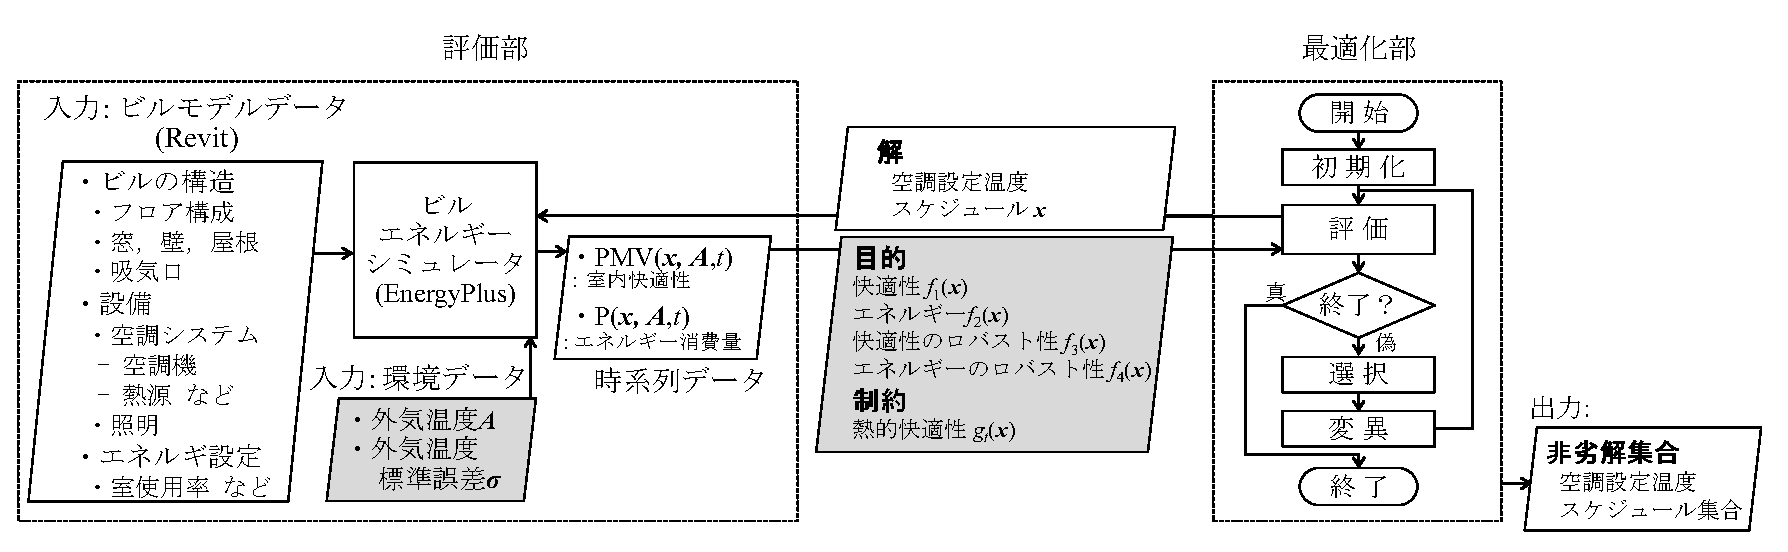
\includegraphics[width=1.1\linewidth]{fig/robust_system.eps}
    \end{center}
    \caption{ロバスト最適化システム}
    \label{fig::robust_system}
\end{figure*}

\section{ロバスト最適化における解評価}
\subsection{過去の予報・実績値に基づくシミュレーション用気温設計}\label{subsec::robust_airtemp}
\subsubsection{過去の気温予報実績の調査}
空調スケジュールの最適化における気温予報誤差を考慮するために,過去の気温実績値および気温予報値を利用する.日本国気象庁の提供する時系列気象予報データ\cite{JMAforecast}および実績データ\cite{JMAactual}を用いる.今回は夏期を対象としており2018年6月~9月のデータを使用して誤差を評価した.気温予報発表時刻は5:00であり,毎日6:00~24:00の予報気温と実際の気温を比較する.\figref{fig::robust_temperror_histogram}に各時刻の予報誤差レベル(実際の気温-予報気温)のヒストグラムを示す.色の違いは時刻の違いを表す.また,\tabref{tab::robust_temperror_statistics}に予報誤差の平均と標準偏差(SD: Standard Deviation)を示す.これらの結果から,各時刻における気温予報誤差は正規分布の傾向にあることがわかる.
一方で,気温予報誤差は各時刻で独立に正規分布で出現するわけではなく,時刻間で依存する傾向があることが知られている.\figref{fig::robust_boxplot}に,(a)最高気温予報が上方誤差を含む日の各時刻における気温予報誤差,(b)最高気温予報が下方誤差を含む日の気温予報誤差の箱ひげ図を示す.この結果から,最高気温予報が上方誤差を含む日は各時刻の誤差も上方に,下方誤差を含む日は各時刻の誤差も下方に出現する傾向がある.そこで,本研究では,\tabref{tab::robust_temperror_statistics}に示すような各時刻$t$における平均$μ_t$・標準偏差$σ_t$を有する正規分布が,上方の予報誤差を生じる場合および下方の予報誤差を生じる場合の2つを取り扱う.


\begin{figure}[t]
    \centerline{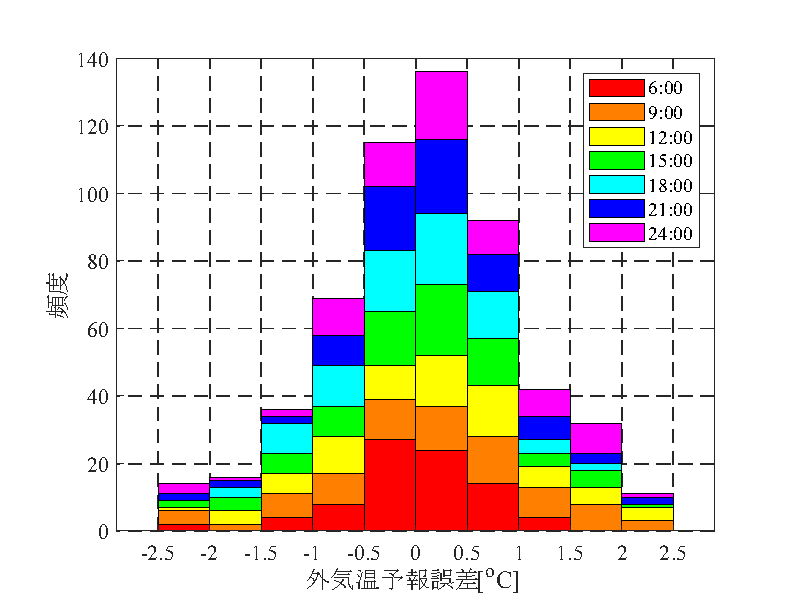
\includegraphics[scale=0.7]{fig/robust_temperror_histogram.eps}}
    \caption{外気温予報誤差のヒストグラム(2018年6~9月, 気象庁発表データ\cite{JMAforecast, JMAactual}をもとに作成)}
    \label{fig::robust_temperror_histogram}
\end{figure}

\begin{figure*}[htbp]
    \begin{center}
        \begin{minipage}{0.7\textwidth}
            \begin{center}
                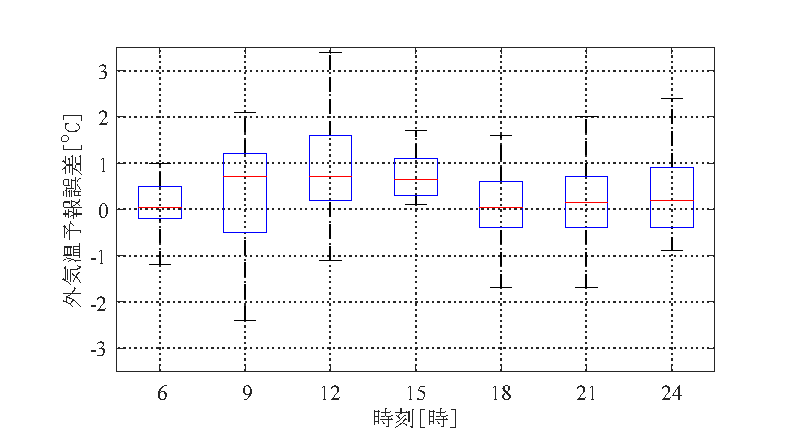
\includegraphics[width=1\textwidth,keepaspectratio=true]{fig/robust_boxplot_upward.eps}\\{\small (a)最高気温予報に上方誤差を含む場合}
            \end{center}
        \end{minipage}
        \\
        \begin{minipage}{0.7\textwidth}
            \begin{center}
                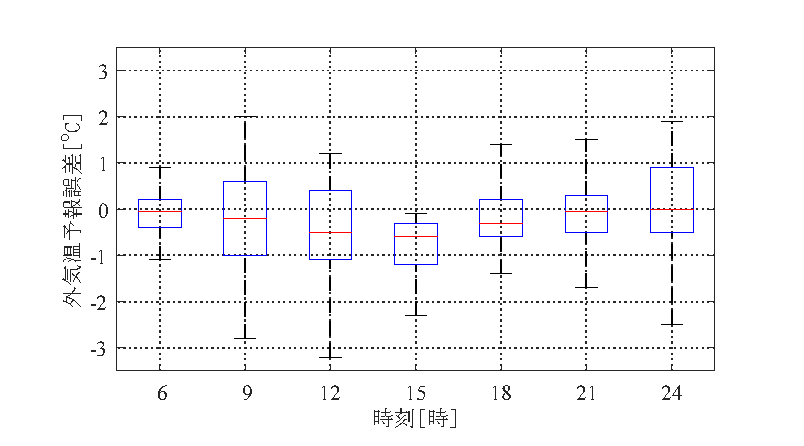
\includegraphics[width=1\textwidth,keepaspectratio=true]{fig/robust_boxplot_downward.eps}\\{\small (b)最高気温予報に下方誤差を含む場合}
            \end{center}
        \end{minipage}
        \vspace{-1mm}
        \caption{外気温予報誤差の箱ひげ図}
        \label{fig::robust_boxplot}
    \end{center}
\end{figure*}

\begin{table}
    \caption{気温予報誤差の統計値}
    \label{tab::robust_temperror_statistics}
    \scalebox{0.85}[0.85]{
        \begin{tabular}{c|c|c|c|c|c|c|c|c}
            \hline
            \textbf{時刻} $t$       & \textbf{6:00} & \textbf{9:00} & \textbf{12:00} & \textbf{15:00} & \textbf{18:00} & \textbf{21:00} & \textbf{24:00} & \textbf{全体} \\
            \hline
            \hline
            平均値$\mu_t$           & -0.0554       & 0.0317        & 0.126          & -0.0448        & -0.134         & -0.08          & -0.00488       & -0.140        \\
            \hline
            標準偏差(SD) $\sigma_t$ & 0.654         & 1.20          & 1.35           & 1.02           & 0.791          & 1.10           & 1.23           & 1.32          \\
            \hline
        \end{tabular}}
\end{table}

\subsubsection{シミュレーション用外気温の設計}
本研究では,気温予報値を$\hat{\mathcal{A}}=\{\hat{a}_{5:00},\hat{a}_{6:00},\dotsc,$ $\hat{a}_{24:00}\}$で表す.ここで$\hat{a}_{t}$は時刻$t\in \{5:00,6:00,\dotsc,24:00\}$における予報気温である.例えば,$\hat{a}_{12:00}=32.0$ [${}^\circ$C]という予報値を示す.気温予報は毎日5:00に発表され,空調設定スケジュールは予報に基づいて最適化される.ビルシミュレータの入力として,気温予報誤差を考慮しない気温を$\mathcal{A}=\{a_{5:00},a_{6:00},\dotsc,$ $a_{24:00}\}$と表す.ここで$a_{t}$は$a_{t}=\hat{a}_{t}+\mu_t$によって得られる時刻$t$における修正された気温である.また,本研究で考慮する気温予報誤差の分散は,多くの誤差発生ケースに対応できるよう$\pm 2\sigma$とする.上方誤差分布を含む気温を$\mathcal{A}^{+2\sigma}=\{a^{+2\sigma}_{5:00},a^{+2\sigma}_{6:00},\dotsc,a^{+2\sigma}_{24:00}\}$,下方誤差分布を含む気温を$\mathcal{A}^{-2\sigma}=\{a^{-2\sigma}_{5:00},a^{-2\sigma}_{6:00},\dotsc,a^{-2\sigma} _{24:00}\}$で表す.時刻$t$における上方予報誤差分布を含む気温$a^{+2\sigma}_t$を以下の式で定義する.

\begin{align}
    \label{eq::robust_airtemp_upward}
    a^{+2\sigma}_t=a_t+2\sigma_t
\end{align}

ここで$\sigma_t$は\tabref{tab::robust_temperror_statistics}における外気温予報誤差の時刻$t$におけるSD値である.同様に,下方予報誤差を含む気温$a^{-2\sigma}_t$を以下の式で定義する.
\begin{align}
    \label{eq:atm2s}
    a^{-2\sigma}_t=a_t-2\sigma_t
\end{align}
\figref{fig::robust_system}で示したように,シミュレーションにおける予報誤差を含まない気温$\mathcal{A}$は,人の室内快適性レベル$f_1$とエネルギー消費量$f_2$の算出に使用される.予報誤差を含む気温$\mathcal{A}^{+2\sigma}$, $\mathcal{A}^{-2\sigma}$は室内快適性とエネルギー消費量のロバスト性を示す目的関数$f_3$, $f_4$の計算に使用される.これらの目的関数の詳細は\secref{sec::robust_objectives}で解説する.

\subsection{設計変数}
本章において,設計変数は\chapref{chap::sim}と同様に,空調設定温度スケジュール$t_{set}(t)$を最適化することとする. 本章では,分割時間間隔$T_s=1$[hour]として,設定可能時刻集合を$\mathcal{T}_{set}=\{6:00, 7:00,\dots, 24:00\}$とする.また設定温度スケジュールを設計変数で表す方法として,\Eqref{eq::sim_variable_diff}を用いる.

\subsection{目的関数}\label{sec::robust_objectives}
本章では,外気温予報に誤差がない場合の室内快適性に関する第1目的関数$f_1$, エネルギー消費量に関する第2目的関数$f_2$に加え,外気温予報に誤差がある場合の快適性の変動幅に関する第3目的関数$f_3$とエネルギー消費量の変動幅に関する第4目的関数$f_4$を考慮する.
\subsubsection{予報誤差のない場合の快適性・エネルギー消費量の評価}
室内快適性に関する第1目的関数$f_1$, エネルギー消費量に関する第2目的関数$f_2$については,\chapref{chap::sim}と同様に予報誤差を考慮しない気温$\mathcal{A}$を用いて,\Eqref{eq::sim_pmv},\eqref{eq::sim_asee}で算出する.

\subsubsection{気温予報誤差がある場合のロバストネスの評価}
目的関数値$f_1$, $f_2$は外気温$\mathcal{A}$の影響を受ける.\subsecref{subsec::robust_airtemp}で述べたように,$f_1$, $f_2$で入力されている$\mathcal{A}$は予報誤差を考慮していない.$\mathcal{A}$と実際の気温に差異がある場合,$\mathcal{A}$に対して最適化された空調スケジュール$\vec{x}$は最適解ではないことがある.快適性レベル$f_1$とエネルギー消費量$f_2$の空調予報誤差の影響を低減するために,本研究では,$f_1$と$f_2$に加えて2つの目的関数の不確実性を考慮する.
第三の目的関数は,上方と下方の予報誤差が発生した場合のビルシミュレーション結果における,予報誤差がない場合との室内快適性レベルの差の最小化とし,以下の目的関数で定式化する.
\begin{align}
    \text{Minimize}~f_3(\vec{x}) & = \max \{|f_1(\vec{x}, \mathcal{A}^{+2\sigma})-f_1(\vec{x}, \mathcal{A})|, |f_1(\vec{x}, \mathcal{A}^{-2\sigma})-f_1(\vec{x}, \mathcal{A})|\}
    \label{eq::robust_objective3}
\end{align}
ここで,$f_1(\vec{x}, \mathcal{A})$は外気温予報が$\mathcal{A}$の場合の室内快適性に関する第1目的関数,$\mathcal{A}^{+2\sigma}$,$\mathcal{A}^{-2\sigma}$は,\subsecref{subsec::robust_airtemp}で述べた上方および下方の誤差分布を含む気温推移である.

同様に,第四の目的関数は,上方と下方の予報誤差が発生した場合のビルシミュレーション結果における,予報誤差がない場合とのエネルギー消費量の差の最小化とし,以下の目的関数で定式化する.

\begin{align}
    \text{Minimize}~f_4(\vec{x}) & = \max \{|f_2(\vec{x}, \mathcal{A}^{+2\sigma})-f_2(\vec{x}, \mathcal{A})|, |f_2(\vec{x}, \mathcal{A}^{-2\sigma})-f_2(\vec{x}, \mathcal{A})|\}
    \label{eq::robust_objective4}
\end{align}

\section{実験内容}
本章では,天気予報誤差によるロバスト性を考慮することの有効性を検証するために2つの手法を比較する.1つめの方法は気温予報誤差を考慮せずに2つの目的関数値$f_1$, $f_2$を最適化する.2つめの方法は,気温予報誤差を考慮して4つの目的関数$f_1$, $f_2$, $f_3$, $f_4$を最適化する.最適化には\subsecref{subsec::OMOPSO}で述べたOMOPSOによって探索する.

\subsubsection{評価シミュレーション部の設定}
本章ではシミュレーションの対象日を\secref{sec::sim_setting}と同様に2006年8月21日の拡張アメダスデータを用い,同じ空調運転モードと設定温度の上下限値を用いる.\figref{fig::robust_outside_temp}に予報誤差を考慮しない気温$\mathcal{A}$および上方・下方の予報誤差を考慮した気温$\mathcal{A}^{+2\sigma}$,$\mathcal{A}^{-2\sigma}$の1日の推移を示す.

\begin{figure}[ht]
    \begin{center}
        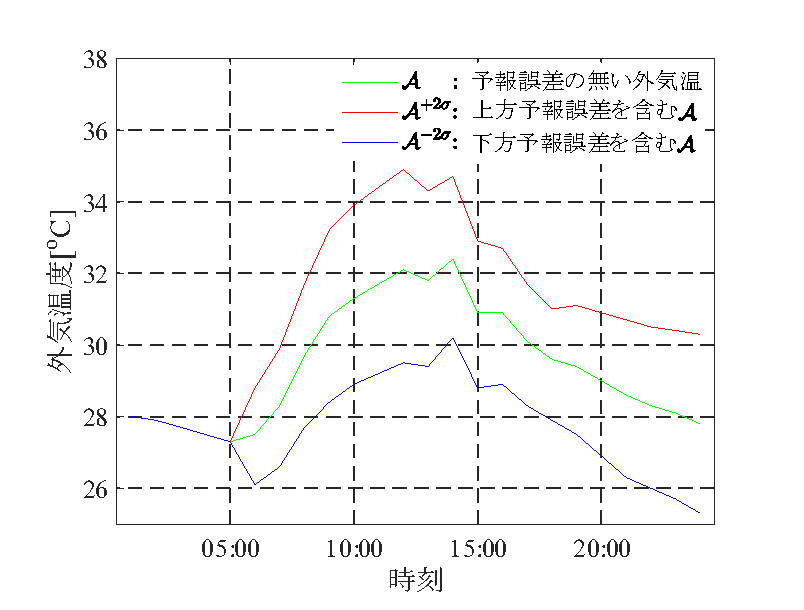
\includegraphics[width=0.7\linewidth]{fig/robust_outside_temp.eps}
    \end{center}
    \caption{シミュレーションに用いた外気温度の推移}
    \label{fig::robust_outside_temp}
\end{figure}

\subsubsection{最適化部の設定}
OMOPSOで用いるパラメータを\tabref{tab::robust_param_omopso}に示す.EnergyPlusシミュレータの実行プログラムとOMOPSOアルゴリズムは\secref{sec::sim_setting}同様Javaで実装した.また,計算の実行にはPCクラスタ(15PC,Windows Server 2012 R2 64ビット,AMD Ryzen7 1800X 3.6GHz, 16GB RAM)を用いた.

\begin{table}[ht]
    {\small
        \begin{center}
            \caption{OMOPSOのパラメータ}
            \label{tab::robust_param_omopso}
            \begin{tabular}{c|cccc}
                \hline
                パラメータ                             & 方法 / 値              \\
                \hline \hline
                ベース粒子群サイズ $N^{\mathcal{P}}$   & 30                     \\
                リーダー粒子群サイズ $N^{\mathcal{L}}$ & 100                    \\
                アーカイブ粒子群サイズ                 & 制限なし               \\
                総世代数 $g_{max}$                     & 500                    \\
                変数長 $n$                             & 19                     \\
                突然変異率 $p_m$                       & $1/n$                  \\
                重み $w$                               & [$0.1, 0.5$)の一様乱数 \\
                重み $c_1, c_2$                        & [$1.5, 2.0$)の一様乱数 \\
                非一様突然変異の係数 $b$               & 5 \cite{Esquivel03}    \\
                $\epsilon$-dominanceの係数$\epsilon$   & 0.0075                 \\
                \hline
            \end{tabular}
        \end{center}
    }
\end{table}

\begin{figure}[htbp]
    \begin{center}
        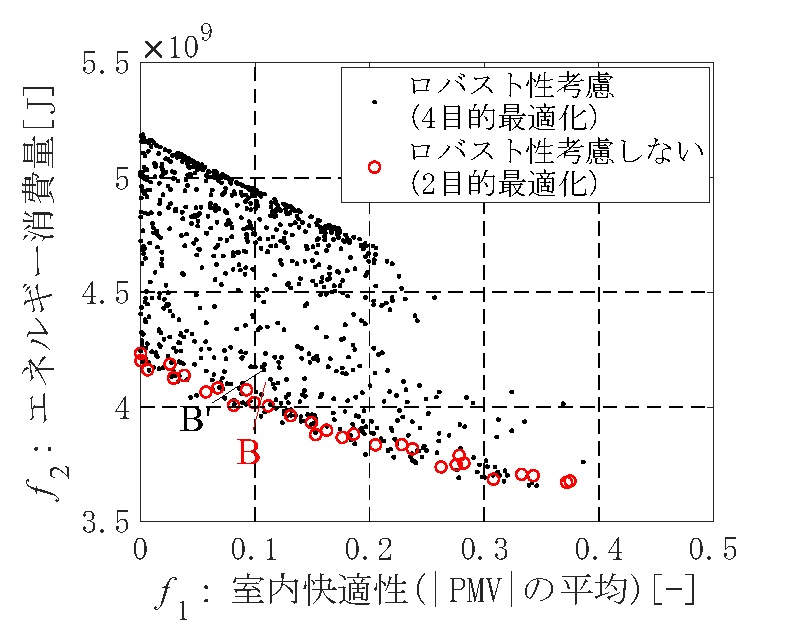
\includegraphics[width=0.7\columnwidth,keepaspectratio=true]{fig/robust_result_pareto_f1f2.eps}\\
        {(a) $f_1$-$f_2$目的関数空間}
    \end{center}
    \begin{center}
        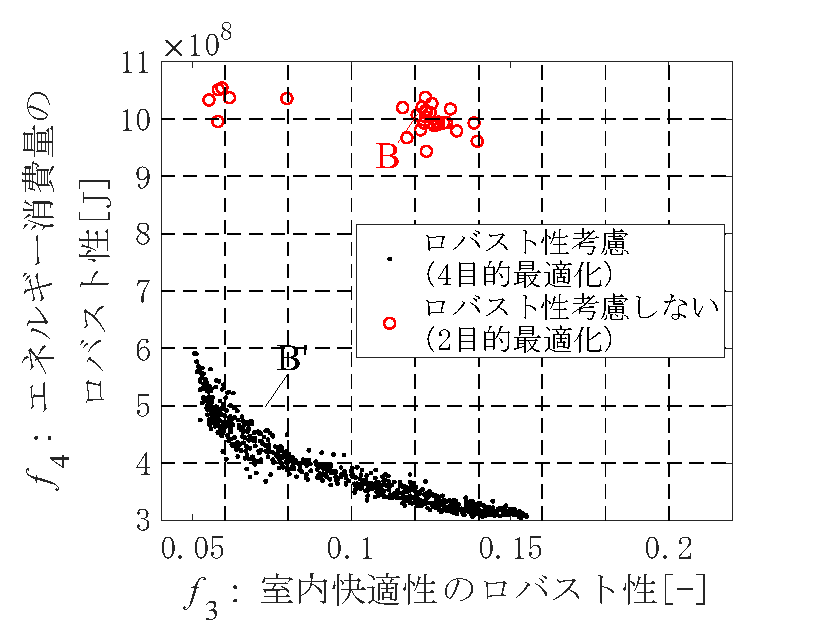
\includegraphics[width=0.7\columnwidth,keepaspectratio=true]{fig/robust_result_pareto_f3f4.eps}\\
        {(b) $f_3$-$f_4$目的関数空間}
    \end{center}
    \caption{ロバスト最適化の結果}
    \label{fig::robust_result_pareto}
\end{figure}

\begin{figure*}[htbp]
    \begin{center}
        \begin{minipage}{.7\textwidth}
            \begin{center}
                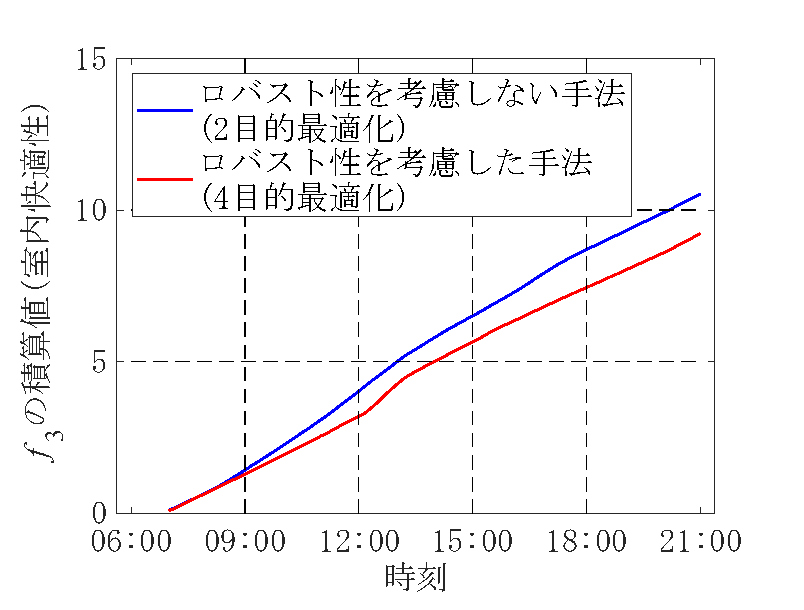
\includegraphics[width=1\textwidth,keepaspectratio=true]{fig/robust_result_schedule_accumulated_comfort.eps}\\\vspace{0.1cm}
                {(a) $f_3$(室内快適性の変動量)の積算値}
            \end{center}
        \end{minipage}
        \begin{minipage}{.7\textwidth}
            \begin{center}
                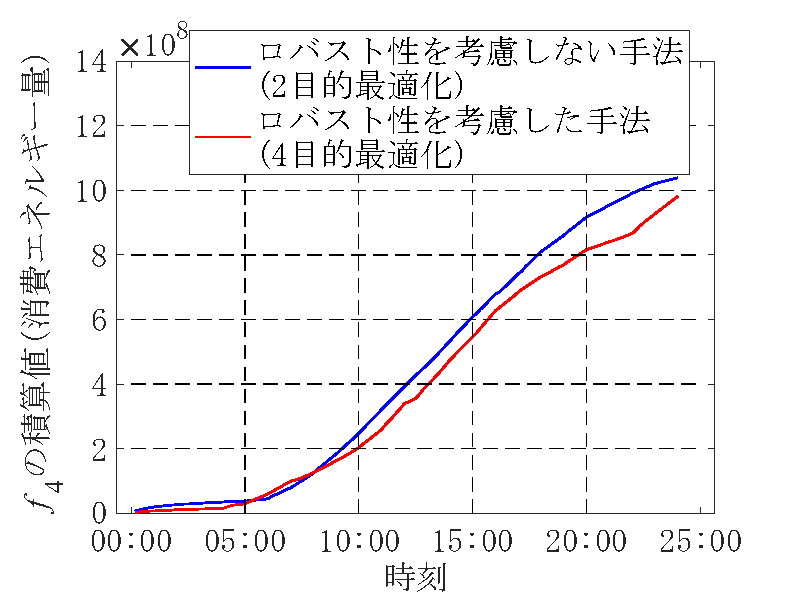
\includegraphics[width=1\textwidth,keepaspectratio=true]{fig/robust_result_schedule_accumulated_power.eps}\\\vspace{0.1cm}
                {(b) $f_4$(エネルギー消費の変動量)の積算値}
            \end{center}
        \end{minipage}
        \vspace{-0.0cm}
        \caption{外気温予報が誤差を含む$\mathcal{A}^{+2\sigma}$と$\mathcal{A}^{-2\sigma}$であった場合の,$f_3$と$f_4$のロバストネス指標値の時間ごとの積算値}
        \label{fig::robust_result_schedule_accumulated}
    \end{center}
\end{figure*}

\section{実験結果と考察}
\subsection{得られた設定温度スケジュール集合の目的関数値}
まず,ロバスト性を考慮せず目的関数値$f_1$と$f_2$を最適化する方法,ロバスト性を考慮して目的関数$f_1$, $f_2$, $f_3$, $f_4$を最適化する方法を比較する.得られた設定温度スケジュール集合を$f_1$, $f_2$目的関数空間上にプロットした結果を\figref{fig::robust_result_pareto} {\bf (a)}に示す.赤点が$f_1$と$f_2$のみを考慮して最適化した結果,黒点がロバスト性に関する目的関数$f_3$と$f_4$も考慮した結果である.$f_1$, $f_2$はそれぞれ小さいほど室内快適性レベル,エネルギー消費量が少なく良好なスケジュールである.

結果から,提案システムにより得られたすべてのスケジュールの室内快適性レベル$f_1$は0.5未満であり,\Eqref{eq::math_constraint_pmv}を満たして実行可能なスケジュールが得られていることがわかる.ロバスト性を考慮しない赤点の結果は30個に対して,ロバスト性を考慮した黒点の結果は880個の解を獲得した.4目的を考慮すると,2目的よりも個々の解の優劣をつけることが困難となり,非劣解となる解が多く発生したためと考える.また,$f_1$, $f_2$を考慮するだけで赤のスケジュールが得られるが,4目的の場合ロバスト性という別の目的関数$f_3$, $f_4$も考慮するため,2目的で探索したほうが目的関数$f_1$,$f_2$でよい値の解の割合が多い.\red{ここで,ロバスト性を考慮しない赤点の2目的最適化とロバスト性を考慮した黒点で示した4目的最適化それぞれで得られたスケジュール集合について,2つの目的関数$f_1$, $f_2$に対するHypervolume値を計算し正規化した結果を\tabref{tab::robust_result_hv}に示す.この結果から,ロバスト性を考慮した4目的最適化の手法では$f_1$, $f_2$目的関数空間で良い解の割合は少ないものの,$f_1$, $f_2$目的関数空間においてもロバスト性を考慮しない2目的最適化と同等かそれより良い解を含んでいる事がわかる.}


\begin{table}[t]
    \begin{center}
        \caption{ロバスト性を考慮しない2目的最適化とロバスト性を考慮した4目的最適化それぞれで獲得した解集合のHypervolume(HV)値}
        \label{tab::robust_result_hv}
        \small
        \begin{tabular}{c|c|c}
            \hline
            手法 & ロバスト性を考慮しない手法(2目的) & ロバスト性を考慮した手法(4目的) \\
            \hline \hline
            HV値 & 0.813                             & 0.866                           \\
            \hline
        \end{tabular}
    \end{center}
\end{table}

同様に,得られた設定温度スケジュール集合を$f_3$, $f_4$目的関数空間上にプロットした結果を\figref{fig::robust_result_pareto} {\bf (b)}に示す.$f_3$と$f_4$は,それぞれ小さいほど外気温の予報誤差による変動を低減できるロバストなスケジュールである.結果から,$f_3$, $f_4$を考慮した黒の点は,赤の点よりも値が小さく良いロバストネスの解を含み,多くの赤の点は,$f_3$, $f_4$の2次元の目的関数空間上で黒の点に優越される.\red{これらの結果から,黒の点で示したロバスト性を考慮した4目的最適化で獲得した設定温度スケジュール集合は,$f_1$, $f_2$目的関数でロバスト性を考慮しない赤の点と同等の解を選択肢として含みつつ,$f_3$, $f_4$で良好であるロバスト性な解を多数探索できていることが分かる.}気温予報はしばしば誤差を含むため,気温予報誤差におけるロバストネスを考慮した空調スケジュールはビル運用において実用的であるといえる.

\red{
    さらに,\figref{fig::robust_result_pareto} {\bf (a)}において4目的最適化で得られた解集合の分布について考察する.4目的最適化によって獲得した解集合は,$f_1 \leq 0.25$の範囲では幅広い範囲に分布しているが,$f_1 \geq 0.25$の範囲では得られている解分布の範囲は狭くなり2目的最適化と同様の解しか得られなくなる.これは,\subsecref{subsec::sim_schedule_timeseries}で述べたような,空調設定スケジュール最適化問題の部分的に多峰性を持つという問題の特徴によるものであると考える.本問題は$f_1$が小さい範囲では多峰性を持ち,異なる設計変数でも類似した目的関数値が得られるため,$f_1$は同様の値でありながらエネルギー消費量$f_2$が悪い値でロバスト性の高い解など,多数存在する多様な解候補を探索できている.これに対し.$f_1$が大きい範囲では制約違反になりやすく設計変数のパターンは類似したものが多くなり,解候補の多様性は低く2目的最適化と同様の値の解しか探索できない.このような傾向があるため,4目的最適化で得られた解集合の分布が$f_1$の範囲によって異なる傾向を持っていると考える.この結果は,上述のようにある最適化問題の各目的関数のロバスト性を目的関数として加えて探索を行うことで,問題の特徴を目的関数空間上の分布として可視化し推測することが可能であることを示唆している.これは,対象とする実世界の最適化問題の難易度を理解するための手法として有効な方法であることが考えられる.
}

\subsection{空調設定スケジュールの時系列分析}
\figref{fig::robust_result_pareto}から2つの得られたスケジュールを抽出し,時系列データの分析を行った.ここでは,ロバストネスを考慮しない2目的最適化の結果から得られたスケジュール$B$と,ロバストネスを考慮した4目的最適化の結果から得られたスケジュール$B'$について着目した.\figref{fig::robust_result_pareto} {\bf (a)}に示すように,$B$と$B’$は$f_1$-$f_2$目的関数空間において近くに位置しているが,一方で\figref{fig::robust_result_pareto} {\bf (b)}に示すように,$f_3$-$f_4$目的関数空間においては$B'$は$B$を優越している.\figref{fig::robust_result_schedule_accumulated} {\bf (a), (b)}に,$B$および$B'$の$f_3$, $f_4$の目的関数値の時間による積算値を示す.両方の図において,小さい値が快適度合いとエネルギー消費量においてロバストであることを示す.この結果から,4目的最適化によって得られた$B'$はロバスト性を考慮していない2目的最適化から得られた$B$に対して$f_3$, $f_4$の積算値が低く,ロバスト性を考慮した提案手法は予報温度誤差による快適度とエネルギー消費量の変動の小さい空調設定温度スケジュールが得られていることがわかる.ロバストな空調設定スケジュールは計画変更の回数を削減でき,月次・年次の電力消費計画を策定するビル管理者にとって実用的である.

\begin{figure*}[htbp]
    \begin{center}
        \begin{minipage}{0.5\textwidth}
            \begin{center}
                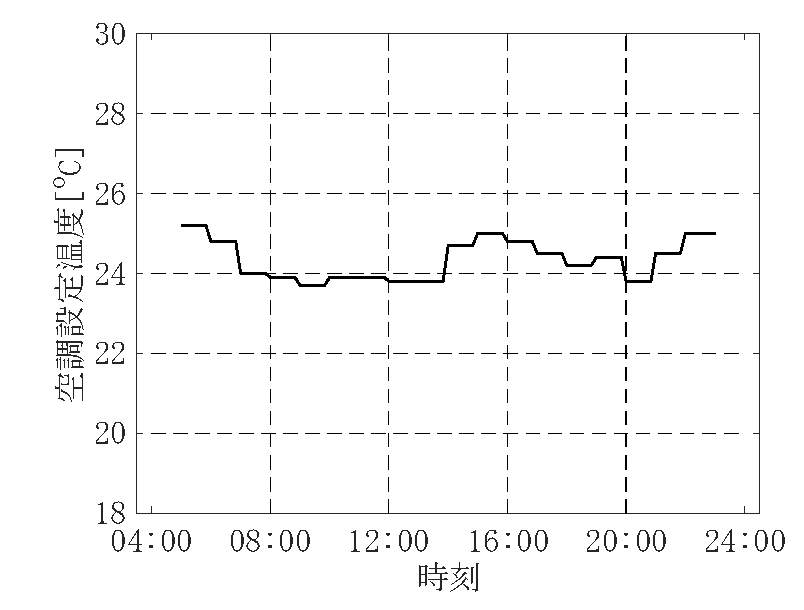
\includegraphics[width=1\textwidth,keepaspectratio=true]{fig/robust_result_schedule_2obj_setting.eps}\\(a) 空調設定温度スケジュール
            \end{center}
        \end{minipage}
        \begin{minipage}{0.5\textwidth}
            \begin{center}
                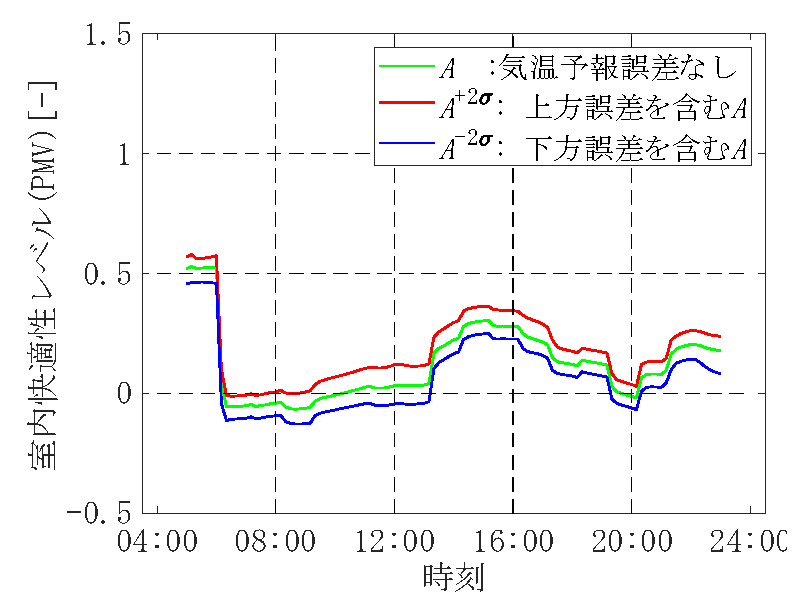
\includegraphics[width=1\textwidth,keepaspectratio=true]{fig/robust_result_schedule_2obj_comfort.eps}\\(b) 室内快適性レベル
            \end{center}
        \end{minipage}
        \begin{minipage}{0.5\textwidth}
            \begin{center}
                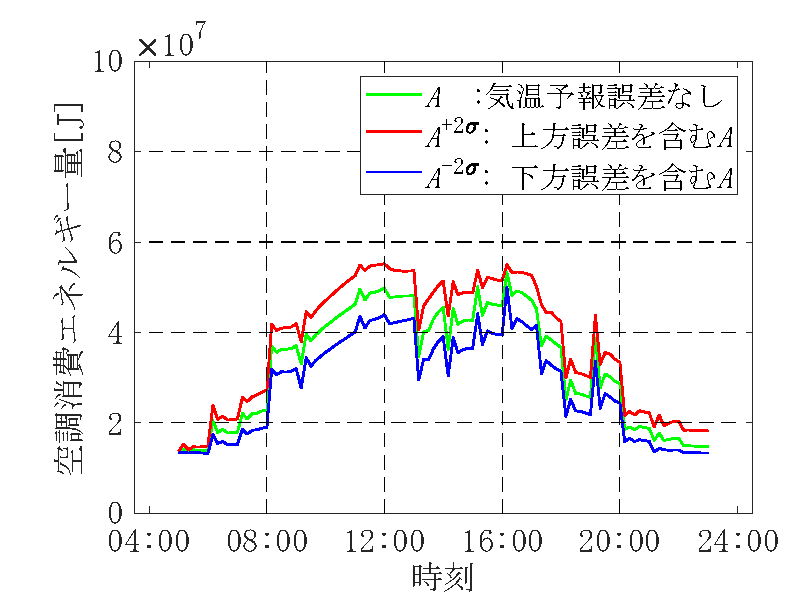
\includegraphics[width=1\textwidth,keepaspectratio=true]{fig/robust_result_schedule_2obj_power.eps}\\(c) エネルギー消費量
            \end{center}
        \end{minipage}
        \caption{ロバスト性を考慮しない2目的最適化で獲得した空調設定スケジュール$B$の時系列データ}
        \label{fig::robust_result_schedule_2obj}
    \end{center}
\end{figure*}

\begin{figure*}[htbp]
    \begin{center}
        \begin{minipage}{0.5\textwidth}
            \begin{center}
                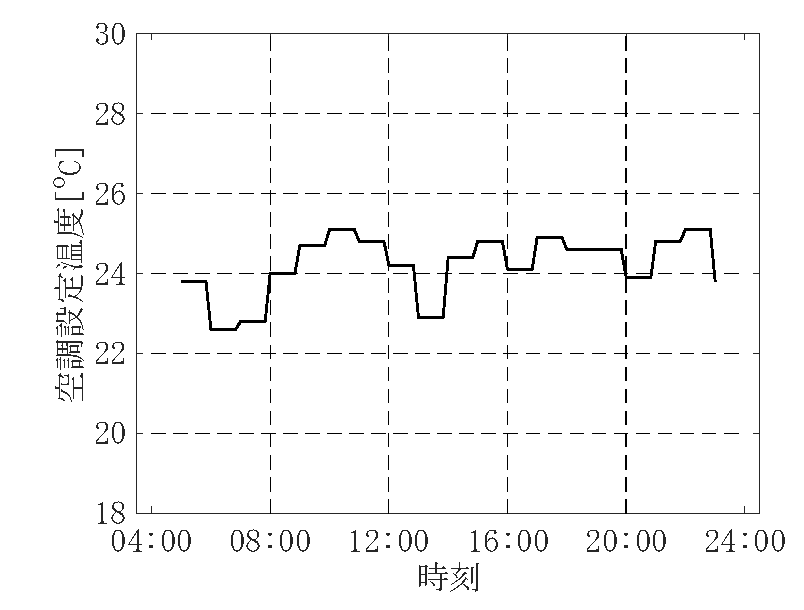
\includegraphics[width=1\textwidth,keepaspectratio=true]{fig/robust_result_schedule_4obj_setting.eps}\\(a)空調設定温度スケジュール
            \end{center}
        \end{minipage}
        \begin{minipage}{0.5\textwidth}
            \begin{center}
                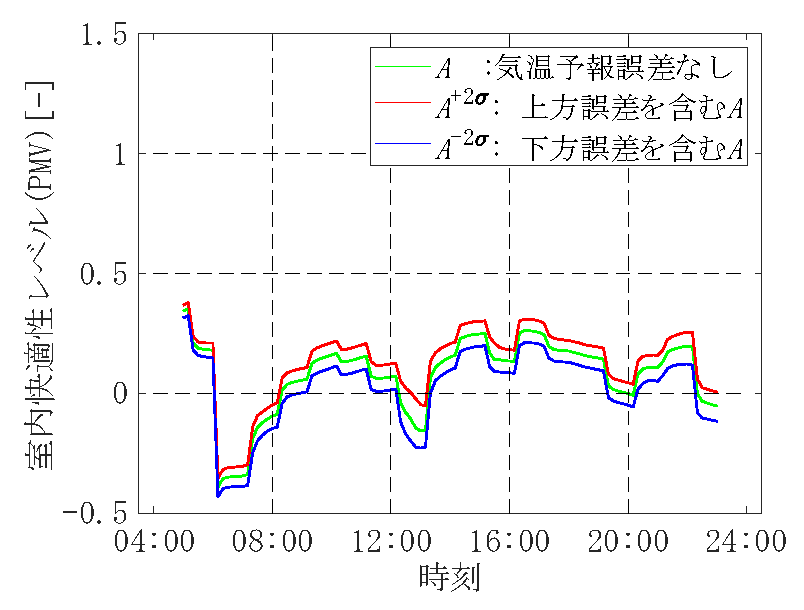
\includegraphics[width=1\textwidth,keepaspectratio=true]{fig/robust_result_schedule_4obj_comfort.eps}\\(b) 室内快適性レベル
            \end{center}
        \end{minipage}
        \begin{minipage}{0.5\textwidth}
            \begin{center}
                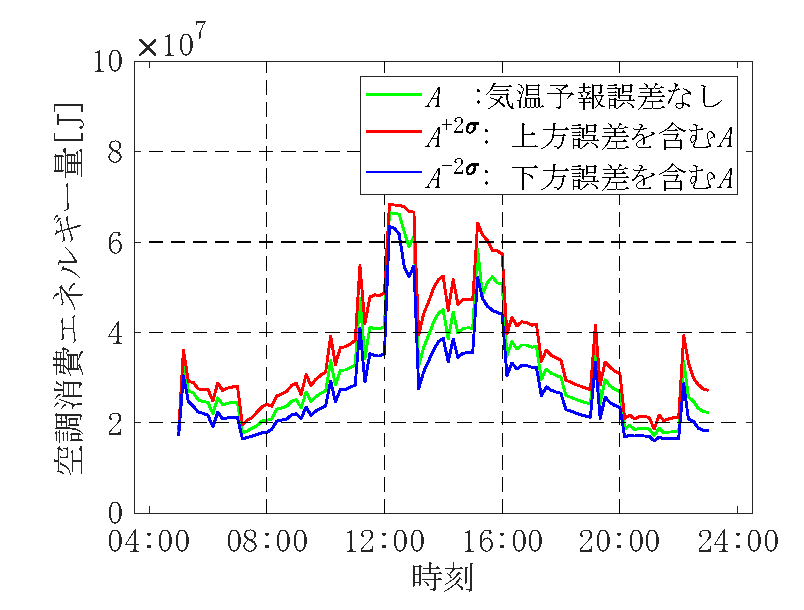
\includegraphics[width=1\textwidth,keepaspectratio=true]{fig/robust_result_schedule_4obj_power.eps}\\(c) エネルギー消費量
            \end{center}
        \end{minipage}
        \caption{ロバスト性を考慮した4目的最適化で獲得した空調設定スケジュール$B'$の時系列データ}
        \label{fig::robust_result_schedule_4obj}
    \end{center}
\end{figure*}

\figref{fig::robust_result_schedule_2obj}と\figref{fig::robust_result_schedule_4obj}に,ロバスト性を考慮していない空調設定スケジュール$B$とロバスト性を考慮した$B’$のスケジュールの,空調設定温度,室内快適性レベル,エネルギー消費量の時系列データをそれぞれ示す.室内快適性およびエネルギー消費量の結果では,緑の線が気温誤差のない場合,赤の線が上方の気温予報誤差がある場合,青の線が下方の気温予報誤差がある場合を示す.\figref{fig::robust_result_schedule_2obj} {\bf (a)}および\figref{fig::robust_result_schedule_4obj} {\bf (a)}から,従来の空調システムは設定温度を1日にわたって一定に保持するのに対し,提案システムは空調設定温度を時間毎に動的に変更していることがわかる.\figref{fig::robust_result_schedule_2obj} {\bf (a)}はロバスト性を考慮しない2目的最適化により得た解$B$のスケジュールであり,設定温度変更幅が小さめである.そのために,\figref{fig::robust_result_schedule_2obj} {\bf (c)}に示すように9:00~13:00と16:00~18:00あたりのエネルギー消費量が気温予報誤差に従って大きく変化してしまっている.
一方,\figref{fig::robust_result_schedule_4obj} {\bf (a)}は不確実性を考慮した4目的最適化で得られた結果$B'$のスケジュールであり,2目的の$B$に比べ設定の変動幅が大きい.結果として,ロバストな解$B'$は,ロバストでない$B$と$f_1$, $f_2$は同程度の値であるにもかかわらず,室内快適性$f_3$およびエネルギー消費量$f_4$の気象予報誤差による変動を低減できている.また,ロバストな解$B'$は昼間の12:00~13:00の時間帯に温度を低く保つことで,効率的に室温を冷やすように運転できている.
ロバスト性を考慮していない温度設定$B$は,気温予報誤差がある場合エネルギー消費量が149[kWh]増加するが,一方ロバスト性を考慮した温度設定$B'$は147[kWh]で済み,気象予報誤差によるエネルギー消費量の増加を1.2\%低減することができている.気温予報はしばしば誤差を含むため,ロバストな空調設定温度スケジュールはビル運用に実用的である.これは,提案した4目的最適化システムがより多様な解を獲得し,ビル管理者に対し提供でき,有用であることを示す.

\subsection{$\pm 2\sigma$以外の気温予報誤差に対するロバスト性の評価}
\subsubsection{目的}
本章で提案した手法では,本章で想定した,各時刻$t$において上方もしくは下方に$2\sigma$の気温予報誤差が発生した場合に対するロバスト性を目的関数とした.前項では,提案したロバスト最適化で獲得したスケジュール集合が,上方もしくは下方に$2\sigma$の誤差が発生した場合に対してロバストであることを示した.一方で,気温予報誤差は必ず$2\sigma$の誤差が発生するというわけではない.その他の気温予報誤差パターンに対しても本手法で獲得したスケジュール集合がロバストであるか,本項で検証する.

\begin{figure}[ht]
    \begin{center}
        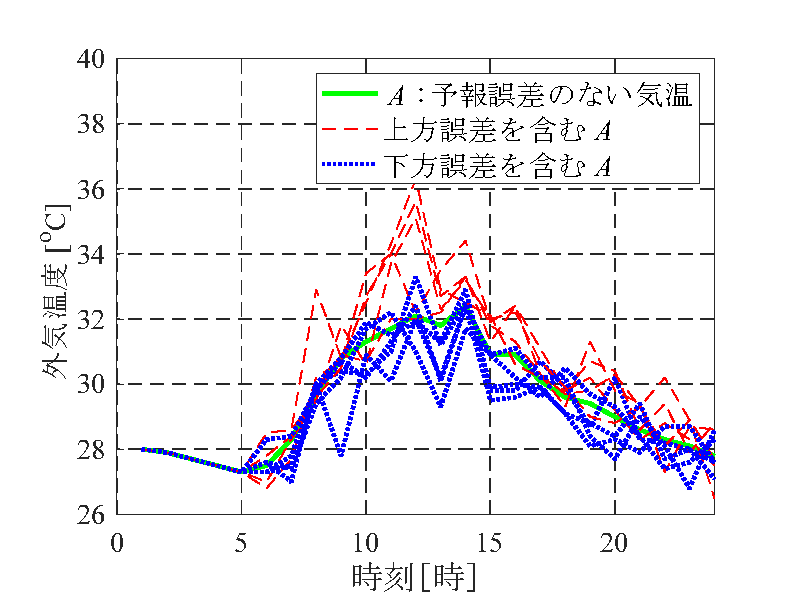
\includegraphics[width=0.7\linewidth]{fig/robust_outside_temp_10.eps}
    \end{center}
    \caption{ロバスト性の評価に用いた外気温予報誤差パターン}
    \label{fig::robust_outside_temp_10}
\end{figure}

\subsubsection{方法}
\subsecref{subsec::robust_airtemp}で述べたとおり,外気温予報誤差の分布はある時刻$t$においては正規分布の傾向にあるが,一方で時刻間での依存関係がある.そこで,正規分布が,上方の予報誤差を生じる場合および下方の予報誤差を生じる場合それぞれで外気温予報誤差パターンを5つずつ生成する.生成した外気温予報誤差パターンを\figref{fig::robust_outside_temp_10}に示す.本図において,緑線が予報誤差のない気温,赤の破線が上方の予報誤差がある気温5パターン,青の点線が下方の予報誤差がある気温5パターンを示す.ロバスト性を考慮しない2目的のシミュレーション最適化で獲得したスケジュール集合と,ロバスト性を考慮した4目的最適化で獲得したスケジュール集合それぞれについて,当日の外気温推移が生成した外気温予報誤差パターンであった場合の室内快適性およびエネルギー消費量の変動幅$f_3$,$f_4$を算出し比較することで,ロバスト性の検証を行う.

\begin{figure*}[htbp]
    \begin{center}
        \begin{minipage}{0.3\textwidth}
            \begin{center}
                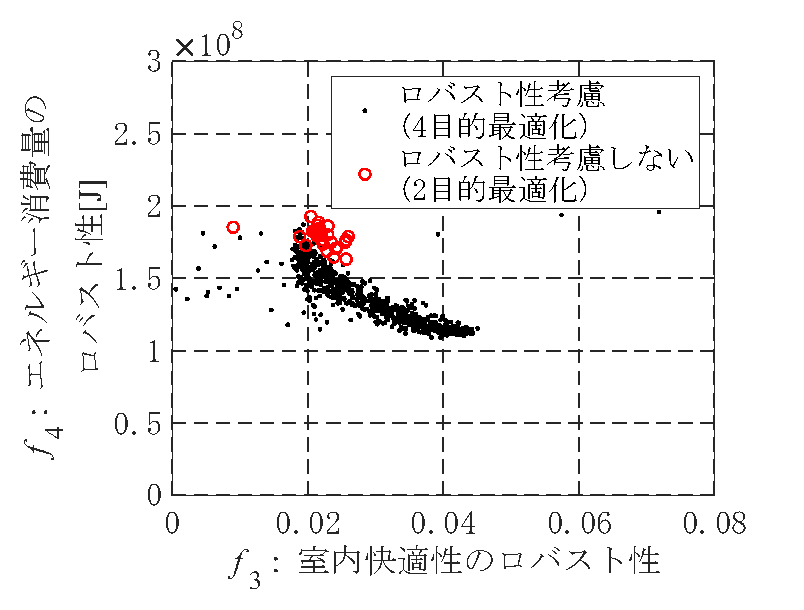
\includegraphics[width=1\textwidth,keepaspectratio=true]{fig/robust_result_pareto_f3f4_10_1.eps}\\\vspace{-3mm}{\small (a)上方誤差があった場合1}
            \end{center}
        \end{minipage}
        \begin{minipage}{0.3\textwidth}
            \begin{center}
                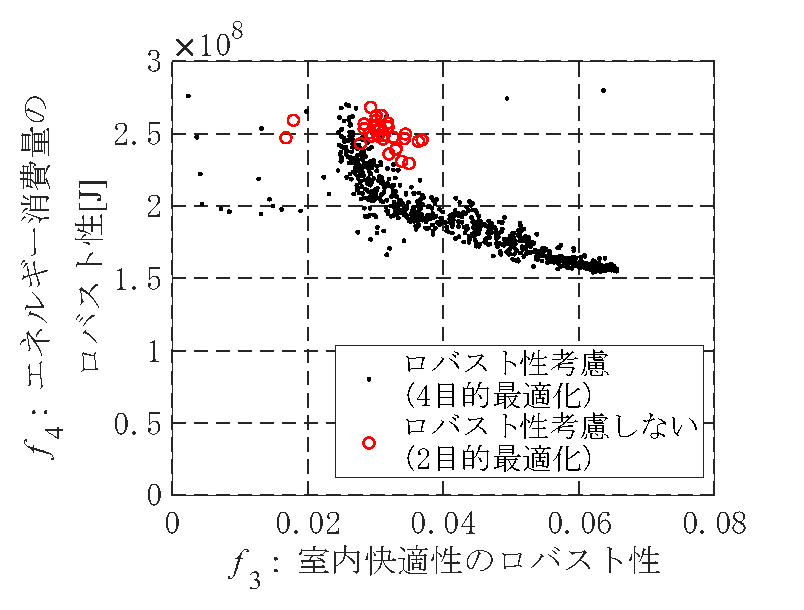
\includegraphics[width=1\textwidth,keepaspectratio=true]{fig/robust_result_pareto_f3f4_10_2.eps}\\\vspace{-3mm}{\small (b)上方誤差があった場合2}
            \end{center}
        \end{minipage}
        \begin{minipage}{0.3\textwidth}
            \begin{center}
                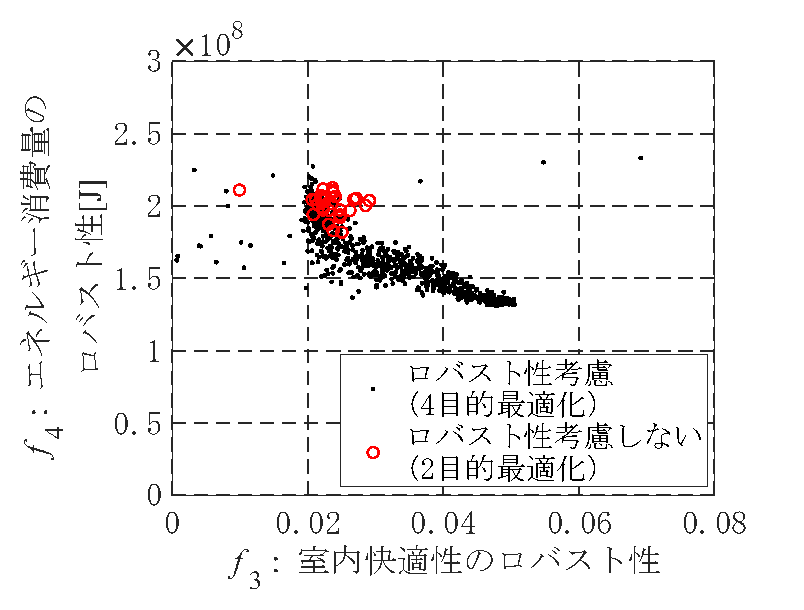
\includegraphics[width=1\textwidth,keepaspectratio=true]{fig/robust_result_pareto_f3f4_10_3.eps}\\\vspace{-3mm}{\small (c)上方誤差があった場合3}
            \end{center}
        \end{minipage}
        \begin{minipage}{0.3\textwidth}
            \begin{center}
                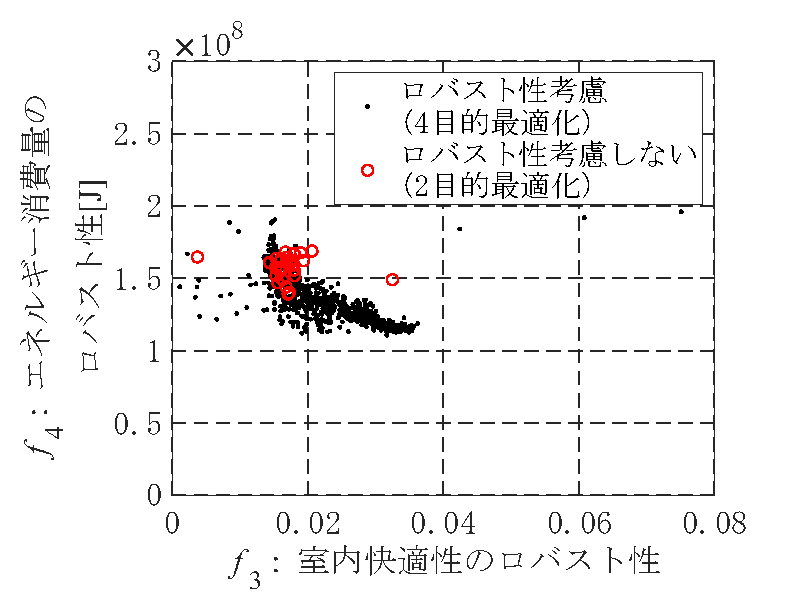
\includegraphics[width=1\textwidth,keepaspectratio=true]{fig/robust_result_pareto_f3f4_10_4.eps}\\\vspace{-3mm}{\small (d)上方誤差があった場合4}
            \end{center}
        \end{minipage}
        \begin{minipage}{0.3\textwidth}
            \begin{center}
                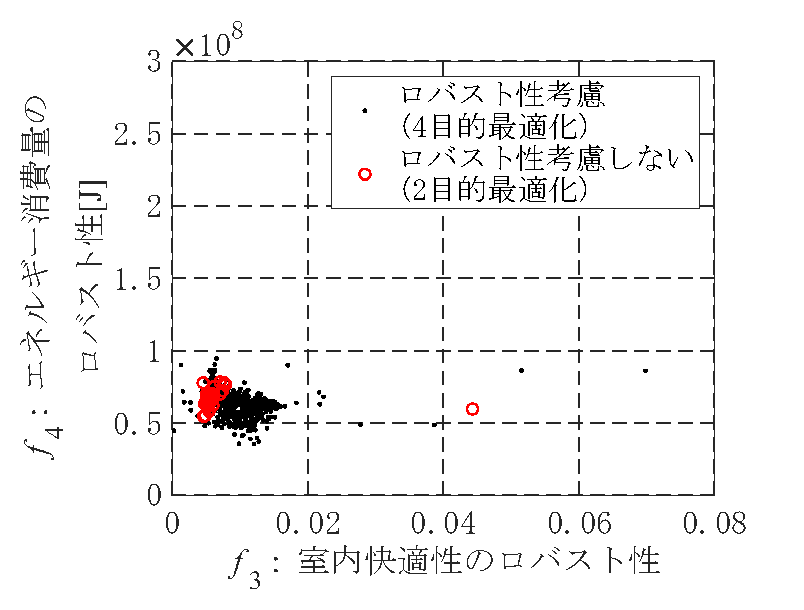
\includegraphics[width=1\textwidth,keepaspectratio=true]{fig/robust_result_pareto_f3f4_10_5.eps}\\\vspace{-3mm}{\small (e)上方誤差があった場合5}
            \end{center}
        \end{minipage}
        \\
        \begin{minipage}{0.3\textwidth}
            \begin{center}
                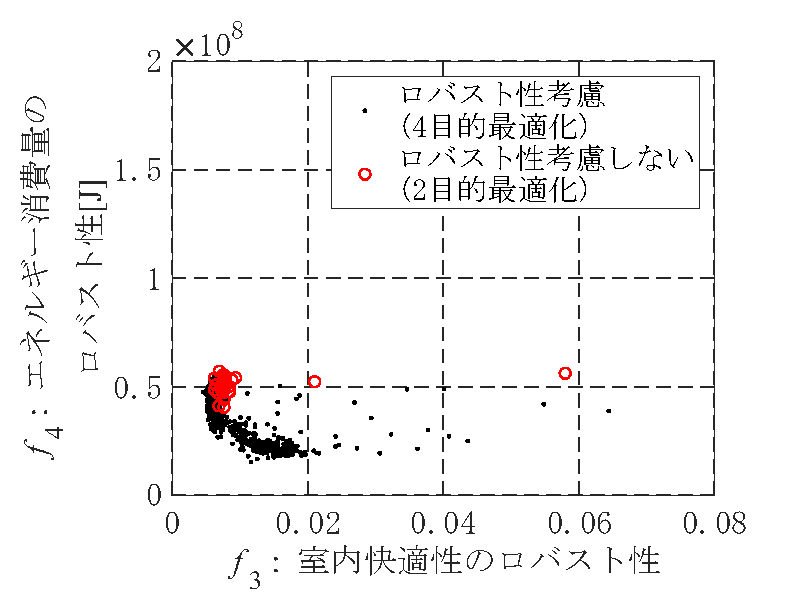
\includegraphics[width=1\textwidth,keepaspectratio=true]{fig/robust_result_pareto_f3f4_10_6.eps}\\\vspace{-3mm}{\small (f)下方誤差があった場合1}
            \end{center}
        \end{minipage}
        \begin{minipage}{0.3\textwidth}
            \begin{center}
                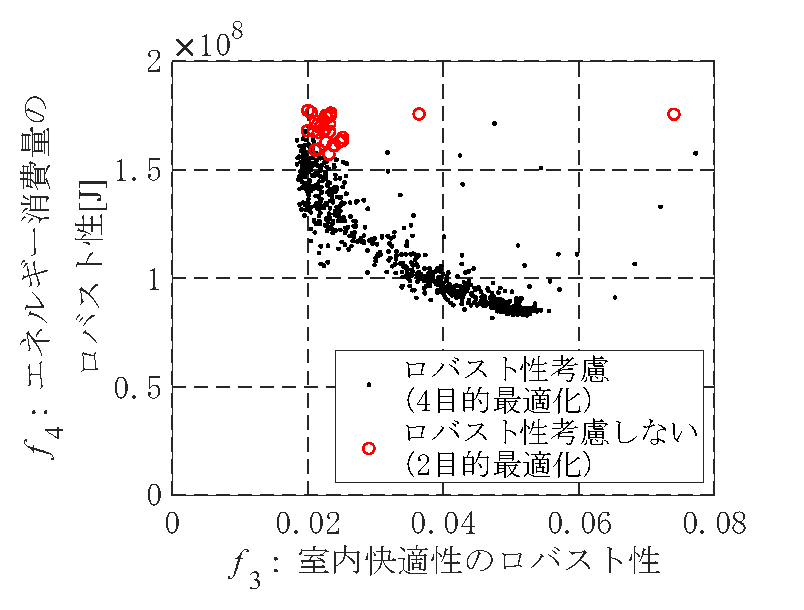
\includegraphics[width=1\textwidth,keepaspectratio=true]{fig/robust_result_pareto_f3f4_10_7.eps}\\\vspace{-3mm}{\small (g)下方誤差があった場合2}
            \end{center}
        \end{minipage}
        \begin{minipage}{0.3\textwidth}
            \begin{center}
                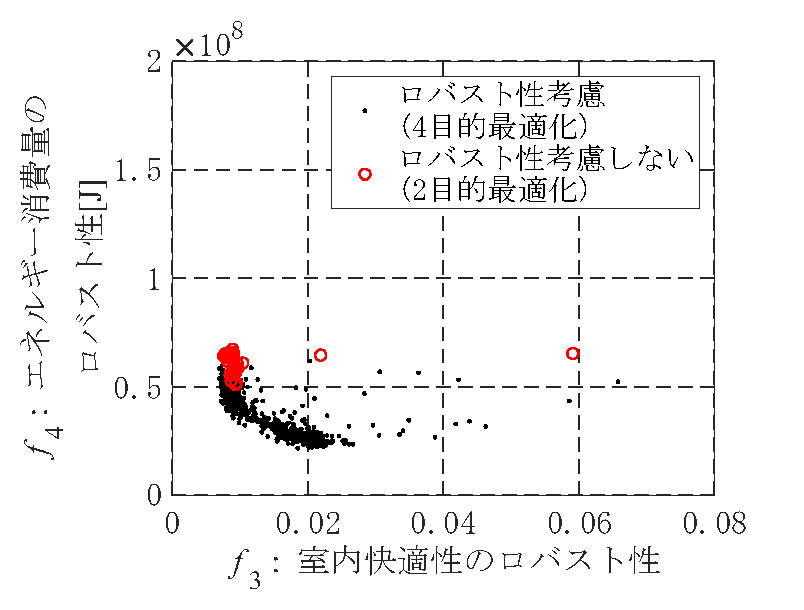
\includegraphics[width=1\textwidth,keepaspectratio=true]{fig/robust_result_pareto_f3f4_10_8.eps}\\\vspace{-3mm}{\small (h)下方誤差があった場合3}
            \end{center}
        \end{minipage}
        \begin{minipage}{0.3\textwidth}
            \begin{center}
                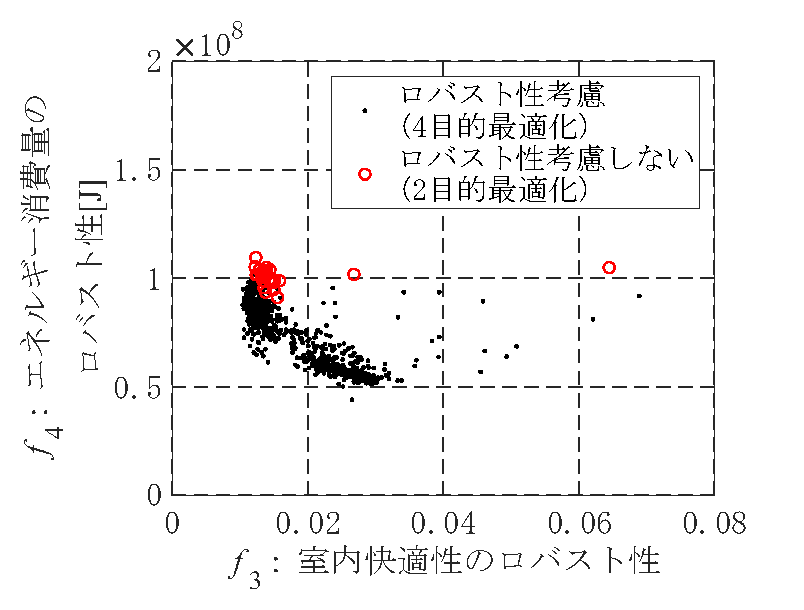
\includegraphics[width=1\textwidth,keepaspectratio=true]{fig/robust_result_pareto_f3f4_10_9.eps}\\\vspace{-3mm}{\small (i)下方誤差があった場合4}
            \end{center}
        \end{minipage}
        \begin{minipage}{0.3\textwidth}
            \begin{center}
                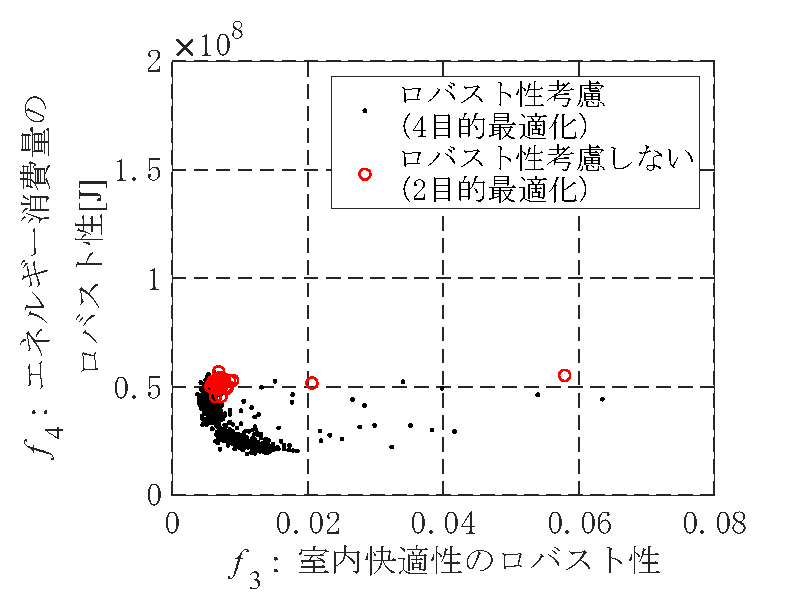
\includegraphics[width=1\textwidth,keepaspectratio=true]{fig/robust_result_pareto_f3f4_10_10.eps}\\\vspace{-3mm}{\small (j)下方誤差があった場合5}
            \end{center}
        \end{minipage}

        \vspace{-1mm}
        \caption{ロバスト性を考慮しない2目的最適化とロバスト性を考慮した4目的最適化で獲得したスケジュール集合の,\figref{fig::robust_outside_temp_10}の気温予報誤差パターンのときのロバスト性}
        \label{fig::robust_result_pareto_10}
    \end{center}
\end{figure*}

\subsubsection{結果}
\figref{fig::robust_outside_temp_10}の外気温予報誤差パターンそれぞれについて,ロバスト性を考慮しない2目的最適化で獲得した解集合と,ロバスト性を考慮した4目的最適化で獲得した解集合のロバスト性に関する目的関数$f_3$,$f_4$を計算した結果を\figref{fig::robust_result_pareto_10}に示す.本結果を見ると,概ねいずれの外気温予報誤差の場合でも,ロバスト性を考慮した4目的最適化によって獲得したスケジュール集合は,ロバスト性を考慮しない2目的最適化によって獲得したスケジュール集合を優越する解分布となっている.\figref{fig::robust_result_pareto_10}(d)~(f)の結果では,2目的最適化と4目的最適化のスケジュール集合は目的関数空間で比較的近くに位置しているが,これは,(d)~(f)の気温の予報誤差が小さいため,快適性およびエネルギー消費量に対して発生する誤差自体も小さかったことが原因であると考えられる.これらの結果から,本章で提案したシステムで獲得したスケジュールは,目的関数でロバスト性の評価に使用した$\pm2\sigma$以外の外気温予報誤差の場合でもロバストであると言える.


\subsection{ロバスト性を考慮した4目的最適化問題に対する多目的進化計算法の選択肢}
\subsubsection{実験内容}
ロバスト性を考慮した本章の最適化問題は,4つの目的関数を含むため,多数目的最適化問題のクラスになる.OMOPSOのようにパレート支配を用いる進化計算は,一般的に,多数目的最適化において性能が悪化する傾向がある.そこで,OMOPSOに加えて,NSGA-II,NSGA-III,MOEA/D-DEによって最適化した結果を比較する.パラメータ設定は,\subsecref{subsec::sim_algo}と同様とした.

\subsubsection{結果}
結果を\figref{fig::robust_result_pareto_algo}に示す.OMOPSO,NSGA-II, MOEA/D-DEは,いずれも良好な目的関数値を示す解を獲得している.OMOPSOは$f_4$,MOEA/D-DEは$f_2$が良い解を獲得している.NSGA-IIIによる解の分布には偏りが見られ,$f_1$, $f_3$は良いが,$f_2$, $f_4$は相対的に良い解が得られない.4種類の手法でそれぞれ獲得した解集合のHV値を\tabref{tab::robust_result_hv_multi}に示す.HVの算出条件は\subsecref{subsec::sim_algo}と同様とした.OMOPSOが最も良いHV値を獲得しており,解分布に偏りのあったNSGA-IIIのHV値が最も悪い値であった.これらの結果から,OMOPSOは,2目的最適化の場合と同様に,ロバスト性を考慮した4目的の多数目的の空調設定スケジュール最適化においても,他のアルゴリズムより良好な解集合が獲得できると考えられる.

\begin{figure}[htb]
    \begin{center}
        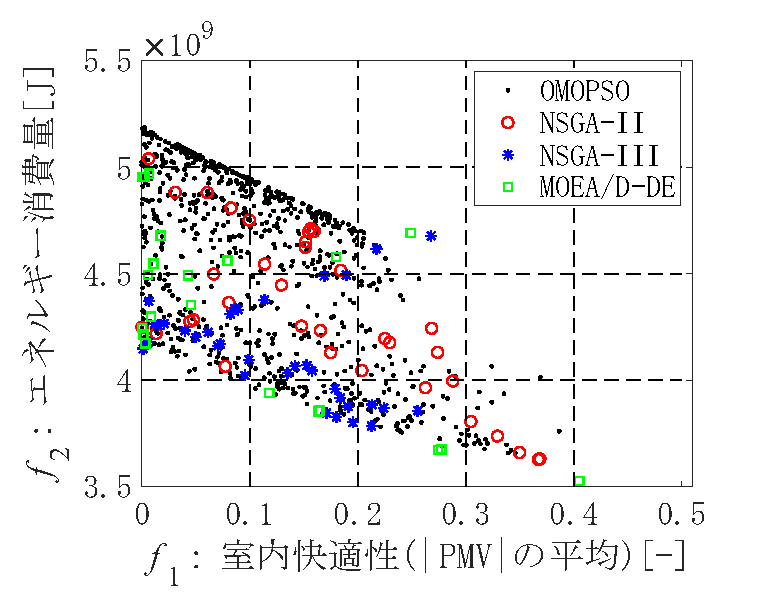
\includegraphics[width=0.7\columnwidth,keepaspectratio=true]{fig/robust_result_algo_pareto_f1f2.eps}\\
        {(a) $f_1$-$f_2$目的関数空間}
    \end{center}
    \begin{center}
        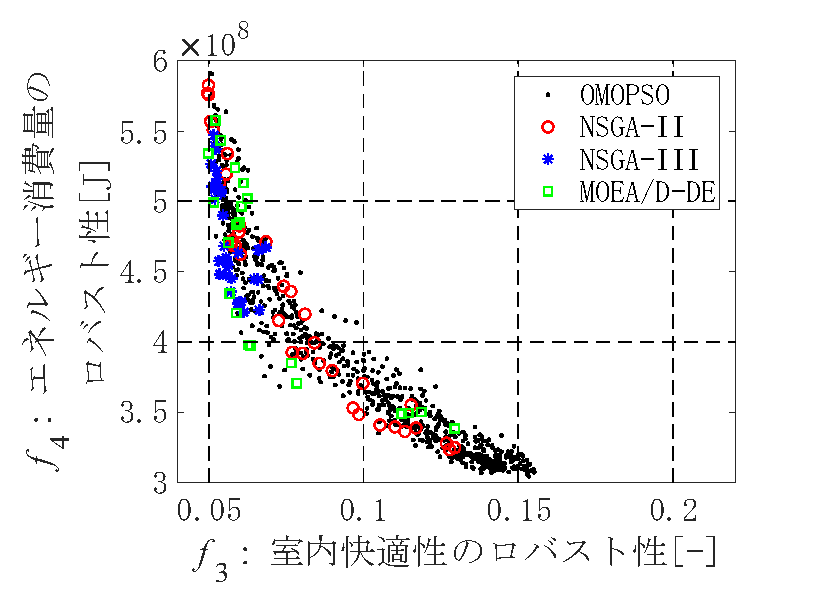
\includegraphics[width=0.7\columnwidth,keepaspectratio=true]{fig/robust_result_algo_pareto_f3f4.eps}\\
        {(b) $f_3$-$f_4$目的関数空間}
    \end{center}
    \caption{4種類の多目的進化計算法によるロバスト最適化の結果}
    \label{fig::robust_result_pareto_algo}
\end{figure}

\begin{table}[t]
    \begin{center}
        \caption{4種類の多目的進化計算法によるロバスト最適化で獲得した解集合のHypervolume(HV)値}
        \label{tab::robust_result_hv_multi}
        \small
        \begin{tabular}{c|c|c|c|c}
            \hline
            手法 & NSGA-II & NSGA-III & MOEA/D-DE & OMOPSO \\
            \hline \hline
            HV値 & 0.578   & 0.481    & 0.587     & 0.643  \\
            \hline
        \end{tabular}
    \end{center}
\end{table}


\subsection{ロバスト性を考慮した4目的最適化問題の他の多数目的最適化ベンチマーク問題との比較}
\subsubsection{実験内容}
ロバスト性を考慮した本章の最適化問題は,4つの目的関数を持つ多数目的最適化問題である.前項ではOMOPSOが本問題に対して有効な性能を示すことが示された.この結果が,他のベンチマーク問題と同様の傾向であるのか,本ロバスト最適化問題に特有の現象であるかを確認するため,ロバスト最適化問題の特徴を分析する.ロバスト最適化問題が既存のベンチマークには無い特徴を有する特殊な問題であれば,特殊なロバスト最適化問題に対してOMOPSOが有効であるという点は従来にない新しい知見であることが確認できる.一方,ロバスト最適化問題が既存のベンチマーク問題に類似していれば,そのベンチマーク問題に対する従来の知見を活用することによりさらに探索性能の高いアルゴリズムが開発できる可能性がある.
本項では,比較対象となる既存のベンチマーク問題の中から多数(4目的以上)の目的関数を持つ最適化問題として,代表的なDTLZテストスイート\cite{Deb05}のうちDTLZ1, 2, 5, 7の4つに加えて,MaF08\cite{Cheng17}, UF12\cite{Zhang08},Water\cite{Ray01}の計7つの問題を取り上げる.これらの最適化ベンチマーク問題に対し,OMOPSOを適用して獲得したパレートフロントの形状から,特徴を分析する.OMOPSOのパラメータは\tabref{tab::robust_param_omopso}と等しくする.多数目的最適化の場合,目的数が4以上となり1つの平面上に解をプロットすることが難しい.そこで,本項では散布図行列を用い,目的関数2つを1対1の散布図としたグラフ目的関数の組合せの数だけ作成して,その特徴を比較することとする.また,空調設定スケジュール最適化問題が4目的であるため,目的数が可変のベンチマーク問題は4目的に設定する.目的数が5目的以上のベンチマーク問題はその目的数で最適化した結果のうち,第1~第4目的の散布図行列をプロットして比較する.

\begin{figure*}[htbp]
    \begin{center}
        \begin{minipage}{0.45\textwidth}
            \begin{center}
                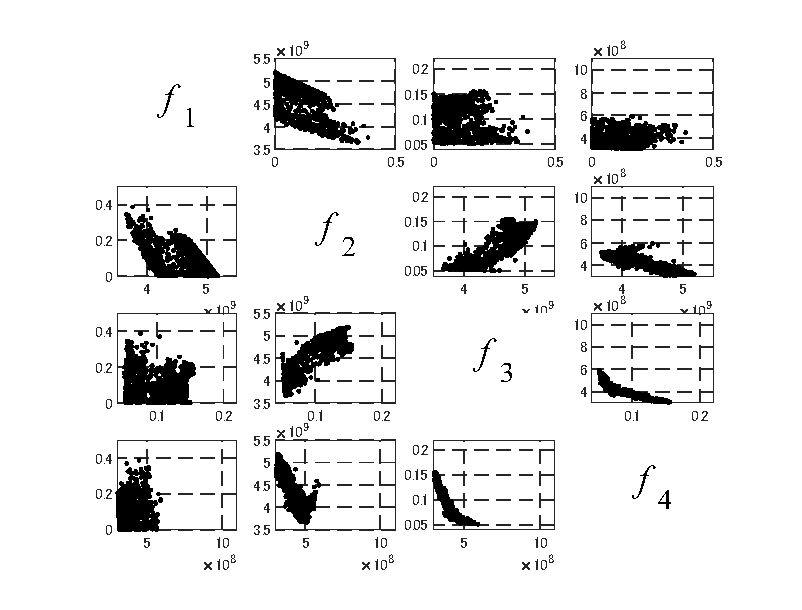
\includegraphics[width=1\textwidth,keepaspectratio=true]{fig/robust_result_pareto_matrix.eps}\\\vspace{-5mm}{\small (a)空調スケジュールロバスト最適化問題}
            \end{center}
        \end{minipage}
        \begin{minipage}{0.45\textwidth}
            \begin{center}
                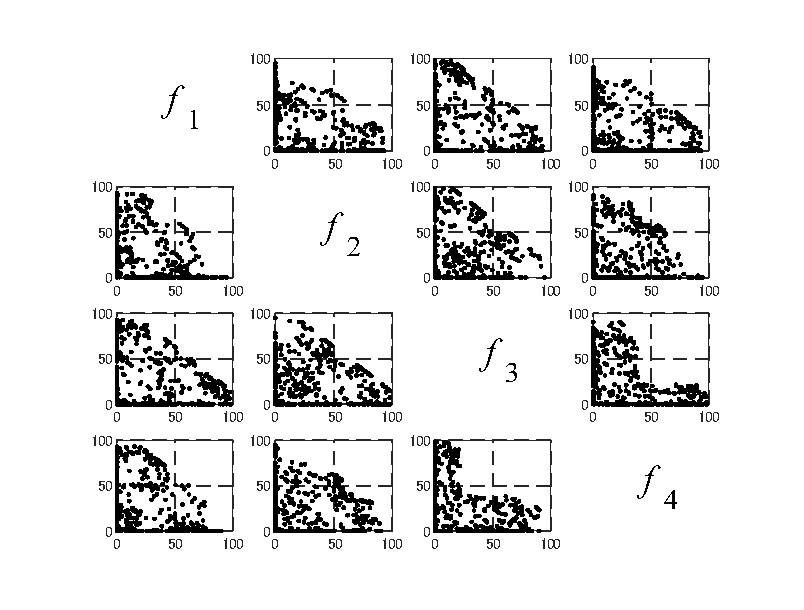
\includegraphics[width=1\textwidth,keepaspectratio=true]{fig/robust_result_pareto_matrix_benchmark_DTLZ1.eps}\\\vspace{-5mm}{\small (b)DTLZ1問題}
            \end{center}
        \end{minipage}
        \begin{minipage}{0.45\textwidth}
            \begin{center}
                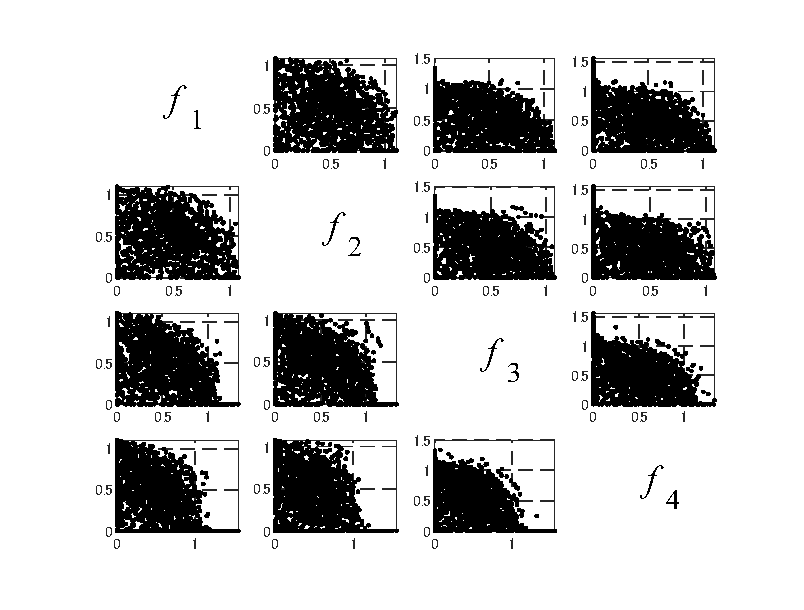
\includegraphics[width=1\textwidth,keepaspectratio=true]{fig/robust_result_pareto_matrix_benchmark_DTLZ2.eps}\\\vspace{-5mm}{\small (c)DTLZ2問題}
            \end{center}
        \end{minipage}
        \begin{minipage}{0.45\textwidth}
            \begin{center}
                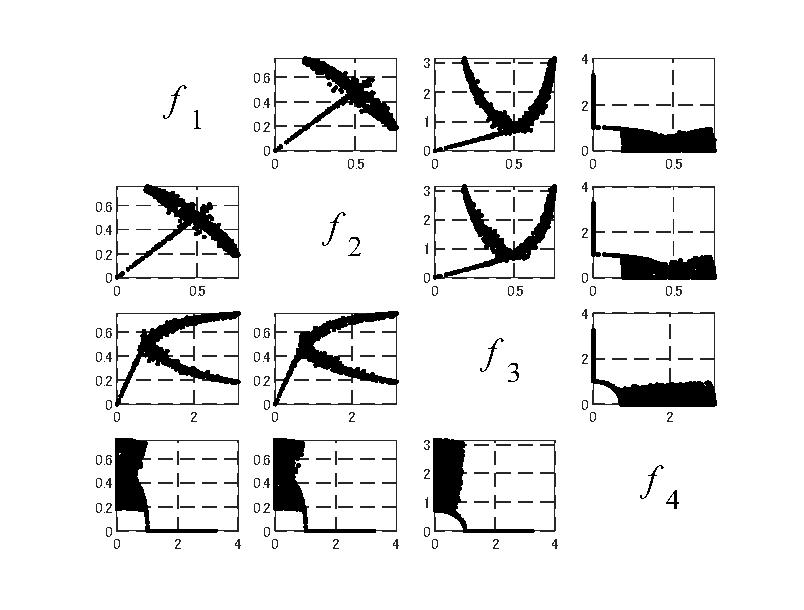
\includegraphics[width=1\textwidth,keepaspectratio=true]{fig/robust_result_pareto_matrix_benchmark_DTLZ5.eps}\\\vspace{-5mm}{\small (d)DTLZ5問題}
            \end{center}
        \end{minipage}
        \begin{minipage}{0.45\textwidth}
            \begin{center}
                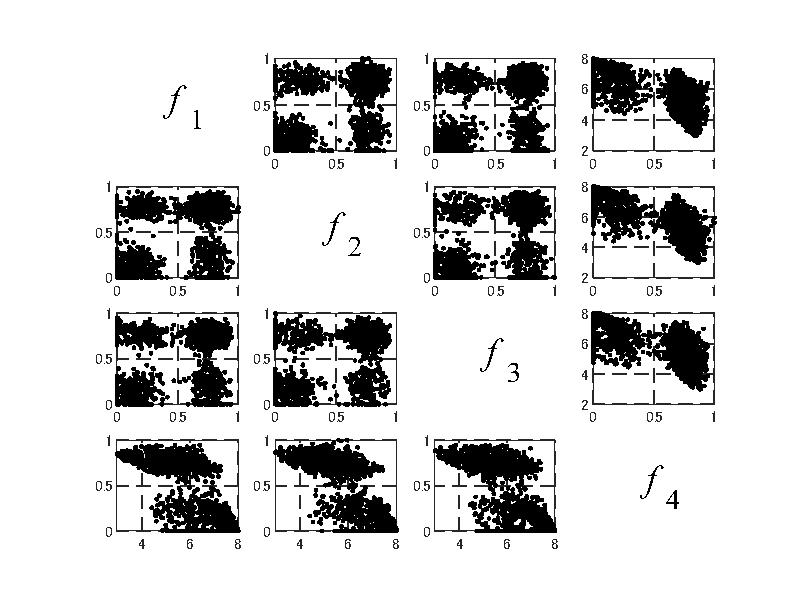
\includegraphics[width=1\textwidth,keepaspectratio=true]{fig/robust_result_pareto_matrix_benchmark_DTLZ7.eps}\\\vspace{-5mm}{\small (e)DTLZ7問題}
            \end{center}
        \end{minipage}
        \begin{minipage}{0.45\textwidth}
            \begin{center}
                \includegraphics[width=1\textwidth,keepaspectratio=true]{fig/robust_result_pareto_matrix_benchmark_MaF08.eps}\\\vspace{-5mm}{\small (f)MaF08問題}
            \end{center}
        \end{minipage}
        \begin{minipage}{0.45\textwidth}
            \begin{center}
                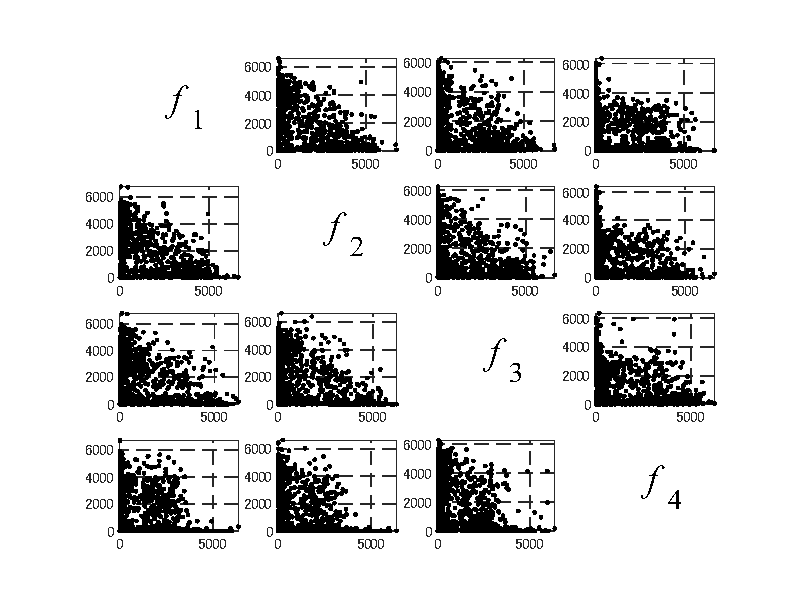
\includegraphics[width=1\textwidth,keepaspectratio=true]{fig/robust_result_pareto_matrix_benchmark_UF12.eps}\\\vspace{-5mm}{\small (g)UF12問題}
            \end{center}
        \end{minipage}
        \begin{minipage}{0.45\textwidth}
            \begin{center}
                \includegraphics[width=1\textwidth,keepaspectratio=true]{fig/robust_result_pareto_matrix_benchmark_Water.eps}\\\vspace{-5mm}{\small (h)Water問題}
            \end{center}
        \end{minipage}

        \vspace{-1mm}
        \caption{ロバスト最適化によって得られた空調設定温度スケジュール集合の目的関数空間における散布図行列}
        \label{fig::robust_result_pareto_matrix}
    \end{center}
\end{figure*}

\subsubsection{結果}
\figref{fig::robust_result_pareto_matrix}に,本章で述べた4目的ロバスト最適化問題と他の7つのベンチマーク問題に対してOMOPSOを適用し,獲得したパレート解集合を散布図行列としてプロットしたものを示す.散布図行列のうち右上側のグラフは,横軸に若い番号の目的関数,縦軸に大きい番号の目的関数の散布図を並べたものであり,左下側はその逆で,横軸に大きい番号,縦軸に若い番号の目的関数を軸にとった散布図を並べたものである.
\figref{fig::robust_result_pareto_matrix}のパレートフロントの散布図行列から,ベンチマーク問題はいくつかのパターンに分類できることがわかる.(b)DTLZ1,(c)DTLZ2,(g)UF12は,いずれも目的関数空間のうち左下半分に解が分布しており,ある2つの目的関数値を同時に小さくすることができるが,残りの目的関数値は大きくなるトレードオフを持つ.(e)DTLZ7,(f)MaF08は目的関数値が取りうる目的関数値が固定的であり,DTLZ7は目的関数空間の4つの象限に別れた円形,MaF08は45°傾斜した半月形になっている.(h)Waterは$f_1-f_3$, $f_2-f_4$間以外の目的関数の間にトレードオフが見られる.(d)DTLZ5は曲線的な特殊なパレートフロント形状を持つ.本章の4目的ロバスト最適化問題で見られたパレートフロント形状(a)は,目的関数によってトレードオフを示すものとそうでないものが混合している点で(f)MaF08問題,(h)Water問題と類似している.一方,パレートフロントが帯状に広がるような分布となっており,分布の広がりが目的関数空間上のエリアによって異なる,といった他のベンチマーク問題には見られない特徴がある.そのため,空調ロバスト最適化問題は他のベンチマークにはない特有の分布形状を持つ問題である可能性があると考えられる.前項でOMOPSOがこの問題に対して有効であることを示したが,この知見が空調設定スケジュールのロバスト最適化に特有の知見であるとすれば,本最適化問題に類似する他の実問題に対してもこの知見が有効である可能性があると考えられる.

\section{結言}
本章では,気象予報誤差に対してロバストな空調設定温度スケジュールの進化型多目的最適化手法を提案した.対象とする建物モデルに対してOMOPSOを使用したシミュレーションベースの進化形多目的最適化を実行し,気温予測に誤差が含まれる場合の室内快適性レベル,エネルギー消費量,およびそれらのロバスト性指標値を最適化した.実験結果は,ロバスト性を考慮した提案システムが温度予報における誤差に対してロバストな,動的に変化する空調温度設定スケジュールを得ることができることを示した.また,OMOPSOは,OMOPSO以外の多目的進化計算法であるNSGA-II,NSGA-III,MOEA/D-DEと比較して良好な解集合を獲得できることを示した.ロバストな空調温度設定スケジュールを含む解集団は,ビル管理者に様々な選択肢を提供し,空調システムの安定した運用とスケジュール変更回数の削減に貢献する.


